The previous chapter began an introduction to the problem of robotic perception, which consists of tasks related to sensing and understanding the robot's own movements as well as the environment in which it operates\cite{SiegwartNourbakhshEtAl2011}. This chapter continues that discussion by diving more deeply into one of the most powerful and challenging tools in robotic perception: computer vision. In particular, this chapter will focus on some of the fundamental mathematical tools for calibrating cameras and processing their images to extract some useful information about the scene\cite{ForsythPonce2011}\cite{HartleyZisserman2002}\nocite{Tsai1987}.
\nocite{Bradski2000}

\notessection{Camera Models and Calibration}
As was discussed in the previous chapter, cameras provide a crucial sensing modality in the context of robotics. This is generally due to the fact that images inherently contain an enormous amount of information about the environment. However, while images do contain a lot of information, extracting the information that is relevant to the robot is quite challenging. One of the most basic tasks related to image processing is determining how a particular point in the scene maps to a point in the camera image, which is sometimes referred to as \textit{perspective projection}. Last chapter, the \textit{pinhole camera model} and the \textit{thin lens model} were presented, and in this chapter the pinhole camera model is leveraged to further explore perspective projection\footnote{All results also hold under the thin lens model, assuming the camera is focused at $\infty$.}.

\begin{figure}[ht]
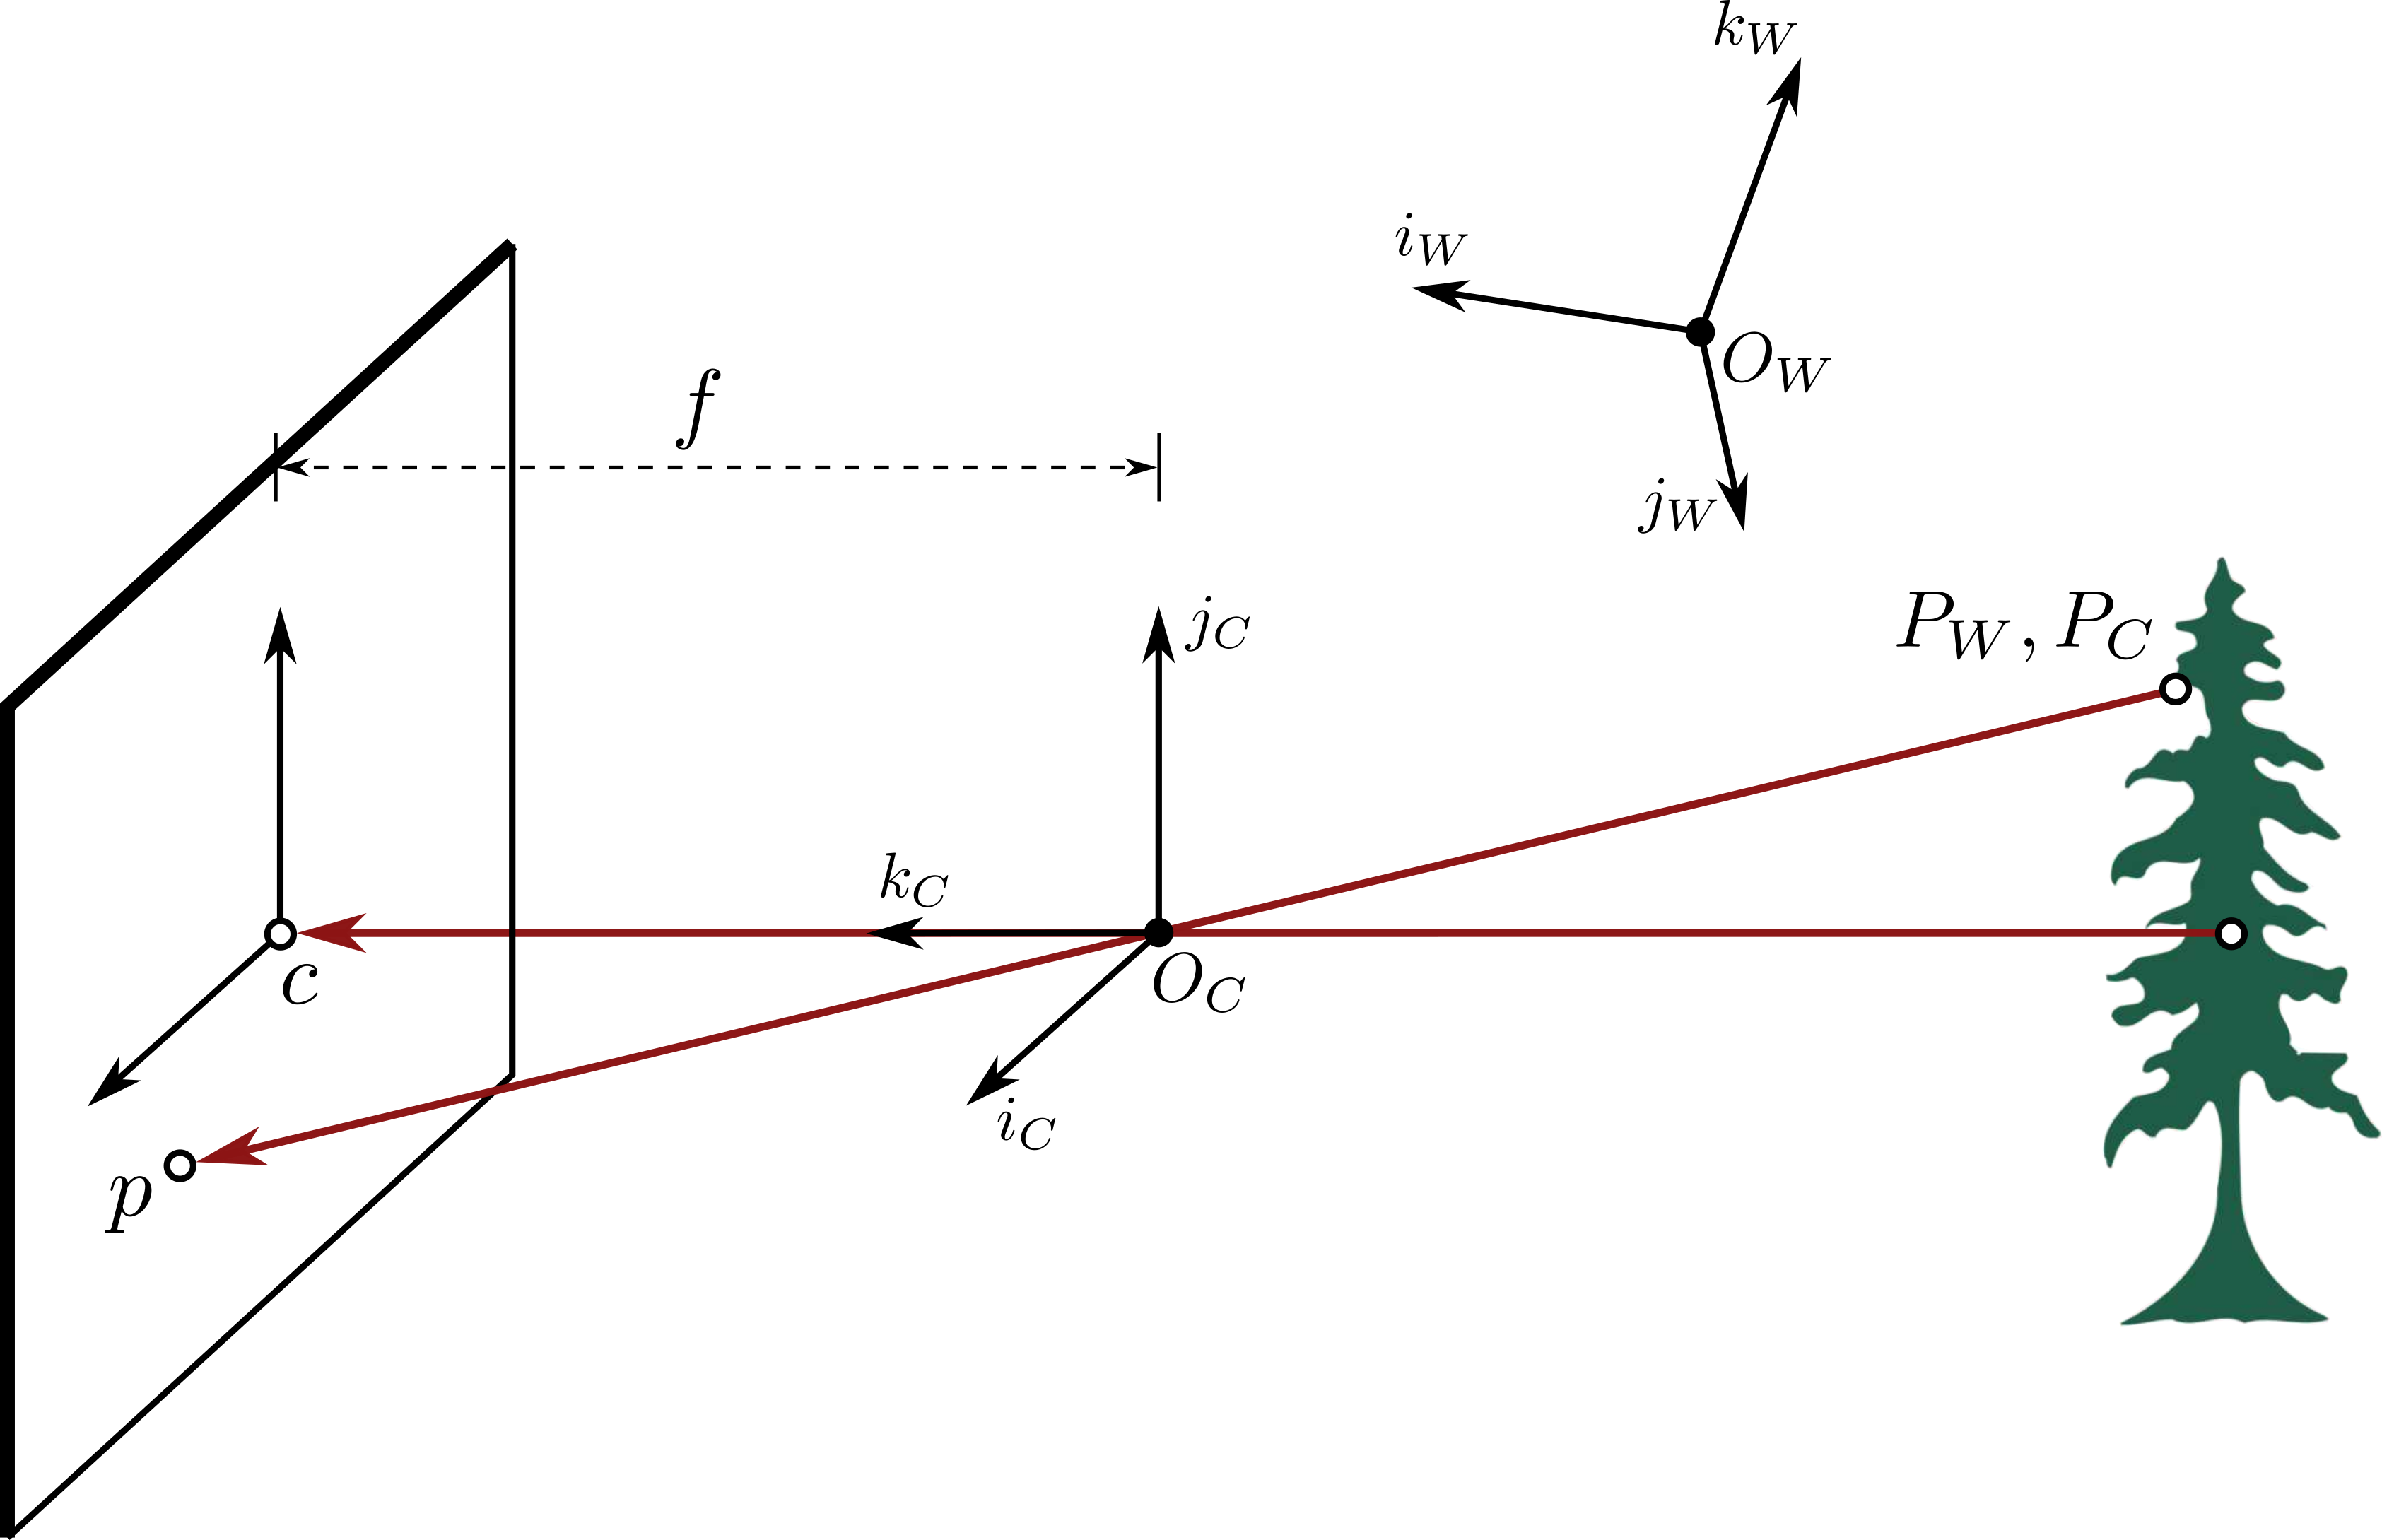
\includegraphics[width=0.8\textwidth]{tex/figs/ch09_figs/pinholecamera2.png}
\centering
\caption{Graphical representation of the pinhole camera model. In this model the point $O_C$ is the camera center, $c$ is the image center, and $f$ is the focal length of the camera. It is assumed that all light rays from point $P$ in the scene pass through point $O_C$ and are captured on the image plane at point $p$.}
\label{fig:pinhole_cam}
\end{figure}

\subsection{Perspective Projection}
The pinhole camera model, shown graphically in Figure \ref{fig:pinhole_cam}, can be used to mathematically define relationships between points $P$ in the scene and points $p$ on the image plane. Notice that any point $P$ in the scene can represented in two ways: in camera frame coordinates (denoted as $P_C$) or in world frame coordinates (denoted as $P_W$). The overall objective of this section is to find derive a mathematical model that can be used to map a point $P_W$ expressed in world frame coordinates to a point $p$ on the image plane. To accomplish this two transformations are combined together, namely a transformation of $P$ from world frame coordinates to camera frame coordinates ($P_W$ to $P_C$) and a transformation from camera coordinates to image coordinates ($P_C$ to $p$).


\subsubsection{Mapping Camera Frame Coordinates to Image Coordinates ($P_C \xrightarrow{} p$)}
The first step considered is the mapping from a point in the scene expressed in camera frame coordinates, $P_C$, to the corresponding point on the image plane, $p$, using the pinhole camera model. Recall from the previous chapter the pinhole camera equations:
\begin{equation} \label{eq:PC2xy}
    x=f\frac{X_C}{Z_C}, \quad  y = f\frac{Y_C}{Z_C},
\end{equation}
where $P_C = (X_C, Y_C, Z_C)$, $p = (x, y)$, and $f$ is the focal length of the pinhole camera\footnote{The $z$ term of $p$ is generally not included simply because $z=f$ is a fixed value.}. 

Note that the quantities $x$ and $y$ are coordinates in the \textit{camera frame}, but it is often desirable to express the point $p$ in terms of \textit{pixel coordinates}. However, pixel coordinates are generally defined with respect to a reference frame in the lower corner of the image plane (to avoid negative coordinates). This new reference frame is shown in Figure \ref{fig:camera_coordinates}, where the image center $c$ is defined in this new reference frame with coordinates $(\tilde{x}_0, \tilde{y}_0)$, where $\tilde{(\cdot)}$ is the notation used to denote a coordinate with respect to this new reference frame.
\begin{figure}[ht]
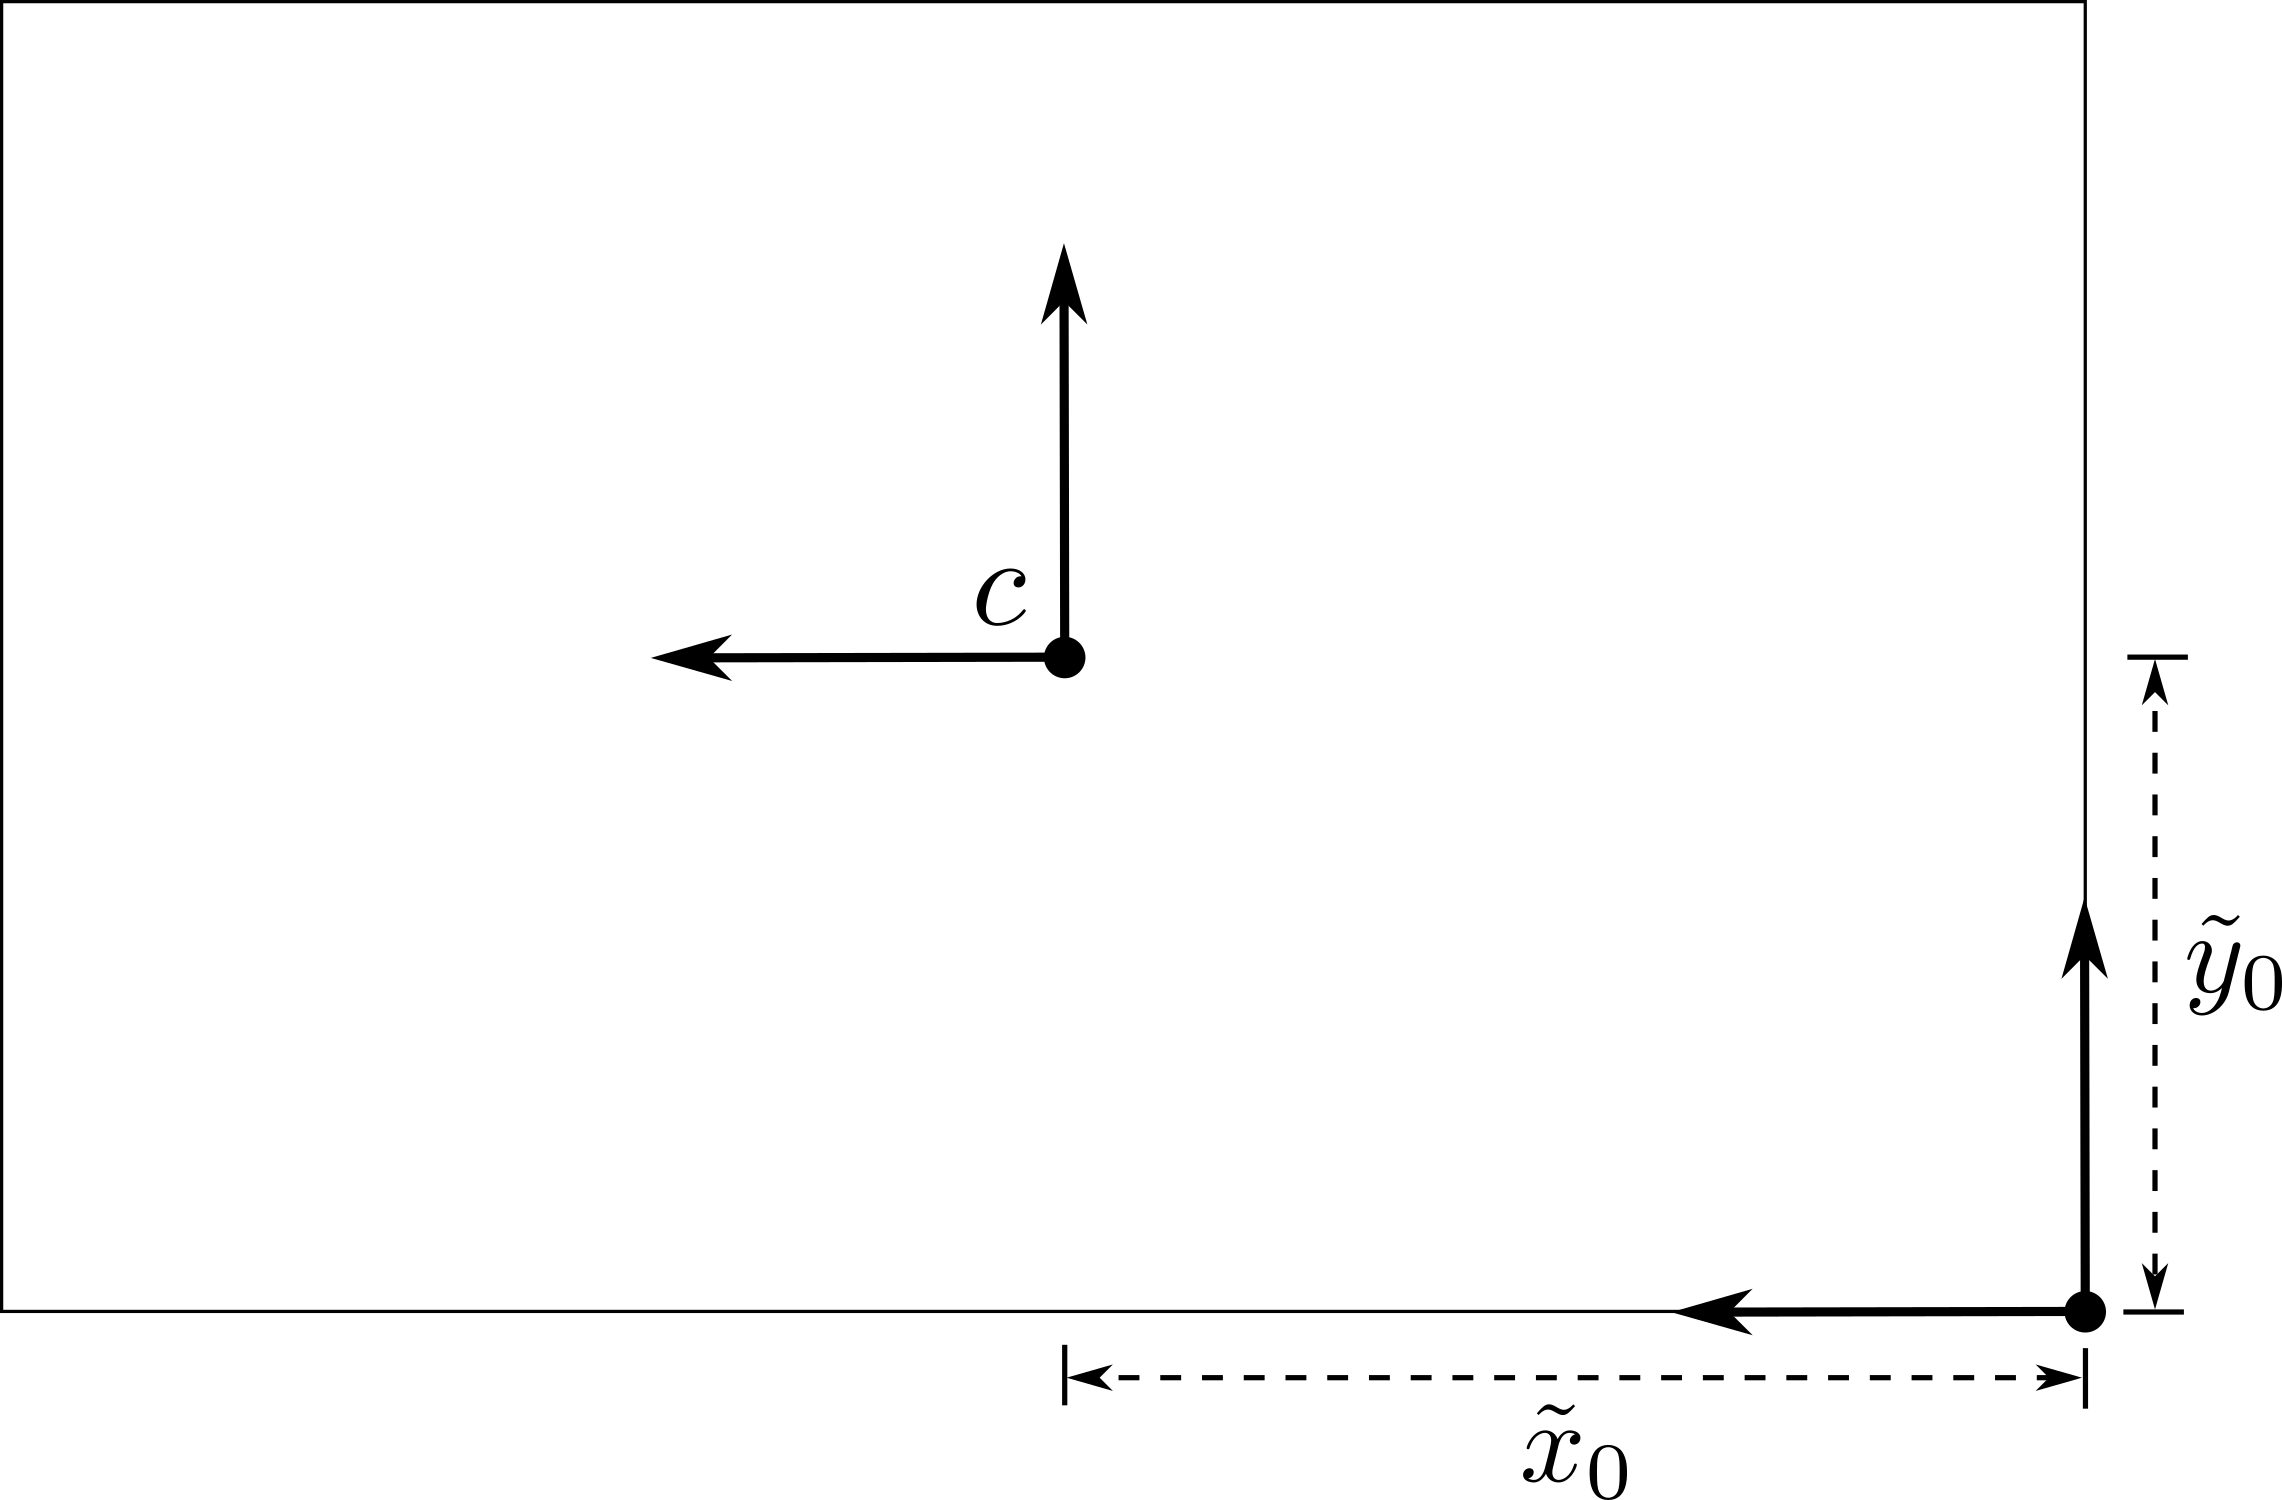
\includegraphics[width=0.55\textwidth]{tex/figs/ch09_figs/imageframe.png}
\centering
\caption{A new reference frame with coordinates denoted by $\tilde{(\cdot)}$  is defined with its origin in the lower corner of the image plane. The image center coordinates in this new frame are denoted $(\tilde{x}_0, \tilde{y}_0)$.}
\label{fig:camera_coordinates}
\end{figure}
In this new reference frame, the point $P_C$ gets mapped to the coordinates $(\tilde{x}, \tilde{y})$ by:
\begin{equation} \label{eq:PC2xtyt}
    \tilde{x} = f\frac{X_C}{Z_C} + \tilde{x}_0, \quad  \tilde{y} = f\frac{Y_C}{Z_C} + \tilde{y}_0.
\end{equation}
Finally, these new coordinates can be mapped to pixel coordinates if the number of pixels per unit distance are known. In particular, the point $P_C$ is mapped to pixel coordinates $(u,v)$ by:
\begin{equation} \label{eq:PC2uv}
   u = \alpha \frac{X_C}{Z_C} + u_0, \quad  v = \beta \frac{Y_C}{Z_C} + v_0,
\end{equation}
where $\alpha = k_xf$, $u_0 = k_x \tilde{x}_0$, $\beta = k_y f$, $v_0 = k_y \tilde{y}_0$, and $k_x$ and $k_y$ are the number of pixels per unit distance in image coordinates.

\paragraph{Homogeneous Coordinates:}
Note that the transformation from the point $P_C$ in camera frame coordinates to $p$ in pixel coordinates given by \eqref{eq:PC2uv} is not linear. However, this transformation can be represented as a linear mapping\footnote{Expressing the perspective projection as a linear map will simplify the mathematics later on.} through an additional change of coordinates. In particular, the points $P_C$ and $p$ will be expressed in \textit{homogeneous coordinates}.

For a 2D point $(x_1,x_2)$ or a 3D point $(x_1,x_2,x_3)$ in Euclidean space, the point can be represented in homogeneous coordinates by the transformation:
\begin{equation}
(x_1,\:x_2) \implies (\alpha x_1, \:\alpha x_2, \:\alpha), \quad \text{and} \quad (x_1,\:x_2,\:x_3) \implies (\alpha x_1,\:\alpha x_2, \:\alpha x_3, \: \alpha),
\end{equation}
for any $\alpha \neq 0$. These new coordinates are called homogeneous coordinates because the scaling factor $\alpha$ can be chosen arbitrarily as long as $\alpha \neq 0$. A set of homogeneous coordinates can then be transformed back by: 
\begin{equation}
(y_1, \: y_2, \:y_3) \implies \Big(\frac{y_1}{y_3}, \: \frac{y_2}{y_3}\Big), \quad \text{and} \quad (y_1,\:y_2,\:y_3,\:y_4) \implies \Big(\frac{y_1}{y_4}, \: \frac{y_2}{y_4}, \: \frac{y_3}{y_4}\Big).
\end{equation}
To denote when a point is described in homogeneous coordinates the superscript $h$ will be used. For example, the point $P_C = (X_C, Y_C, Z_C)$ in camera frame coordinates can be expressed by:
\begin{equation*}
    P_C^h = (X_C, Y_C, Z_C, 1),
\end{equation*}
by choosing $\alpha = 1$, and the point $p = (u,v)$ in pixel coordinates can be expressed in homogeneous coordinates by:
\begin{equation*}
    p^h = (Z_C u, \: Z_C v, \:Z_C) = (\alpha X_C + u_0 Z_C, \: \beta Y_C + v_0 Z_C),
\end{equation*}
by choosing $\alpha = Z_C$ and substituting the expressions \eqref{eq:PC2uv}. With the expression of these points in homogeneous coordinates it can be seen that their relationship is transformed from the nonlinear relationship \eqref{eq:PC2uv} to the \textit{linear} relationship:
\begin{equation}
\begin{bmatrix}
\alpha & 0 & u_{0} & 0 \\
0 & \beta & v_{0} & 0  \\
0 & 0 & 1 & 0
\end{bmatrix}
\begin{pmatrix}
X_{c} \\
Y_{c} \\
Z_{c} \\
1
\end{pmatrix}
=
\begin{pmatrix}
\alpha X_{c} + u_{0}Z_{c} \\
\beta Y_{c} + v_{0}Z_{c} \\
Z_{c} \\
\end{pmatrix}.
\end{equation}

Often in practice a skewness parameter $\gamma$ is also added (which generally ends up being close to 0), and this relationship can be written in the more compact form:
\begin{equation} \label{eq:PC2uvhomo}
    \begin{bmatrix}
        K & 0_{3 \times 1}
    \end{bmatrix} P_C^h = p^h, \quad K = \begin{bmatrix}
\alpha & \gamma & u_{0} \\
0 & \beta & v_{0}  \\
0 & 0 & 1
\end{bmatrix}.
\end{equation}
The matrix $K$ defined in \eqref{eq:PC2uvhomo} is sometimes referred to as the \textit{camera matrix} or \textit{matrix of intrinsic parameters}. It is referred to in this way because it contains the five parameters that define the fundamental characteristics of the camera (from the perspective of the pinhole camera model). While these parameters may be specified by the camera manufacturer, they are often extracted by performing a camera calibration.


\subsubsection{Mapping World Coordinates to Camera Coordinates ($P_W \xrightarrow{} P_C$)}
Recall from Figure \ref{fig:pinhole_cam} that a point $P$ in the scene can either be expressed in terms of camera frame coordinates $P_C$ or world frame coordinates $P_W$. While the previous section discussed the use of the pinhole model to map $P_C$ coordinates to pixel coordinates $p$, this section will discuss the mapping between the camera and world frame coordinates of the point $P$ (see Figure \ref{fig:Pc2Pw}).
\begin{figure}[ht]
\centering
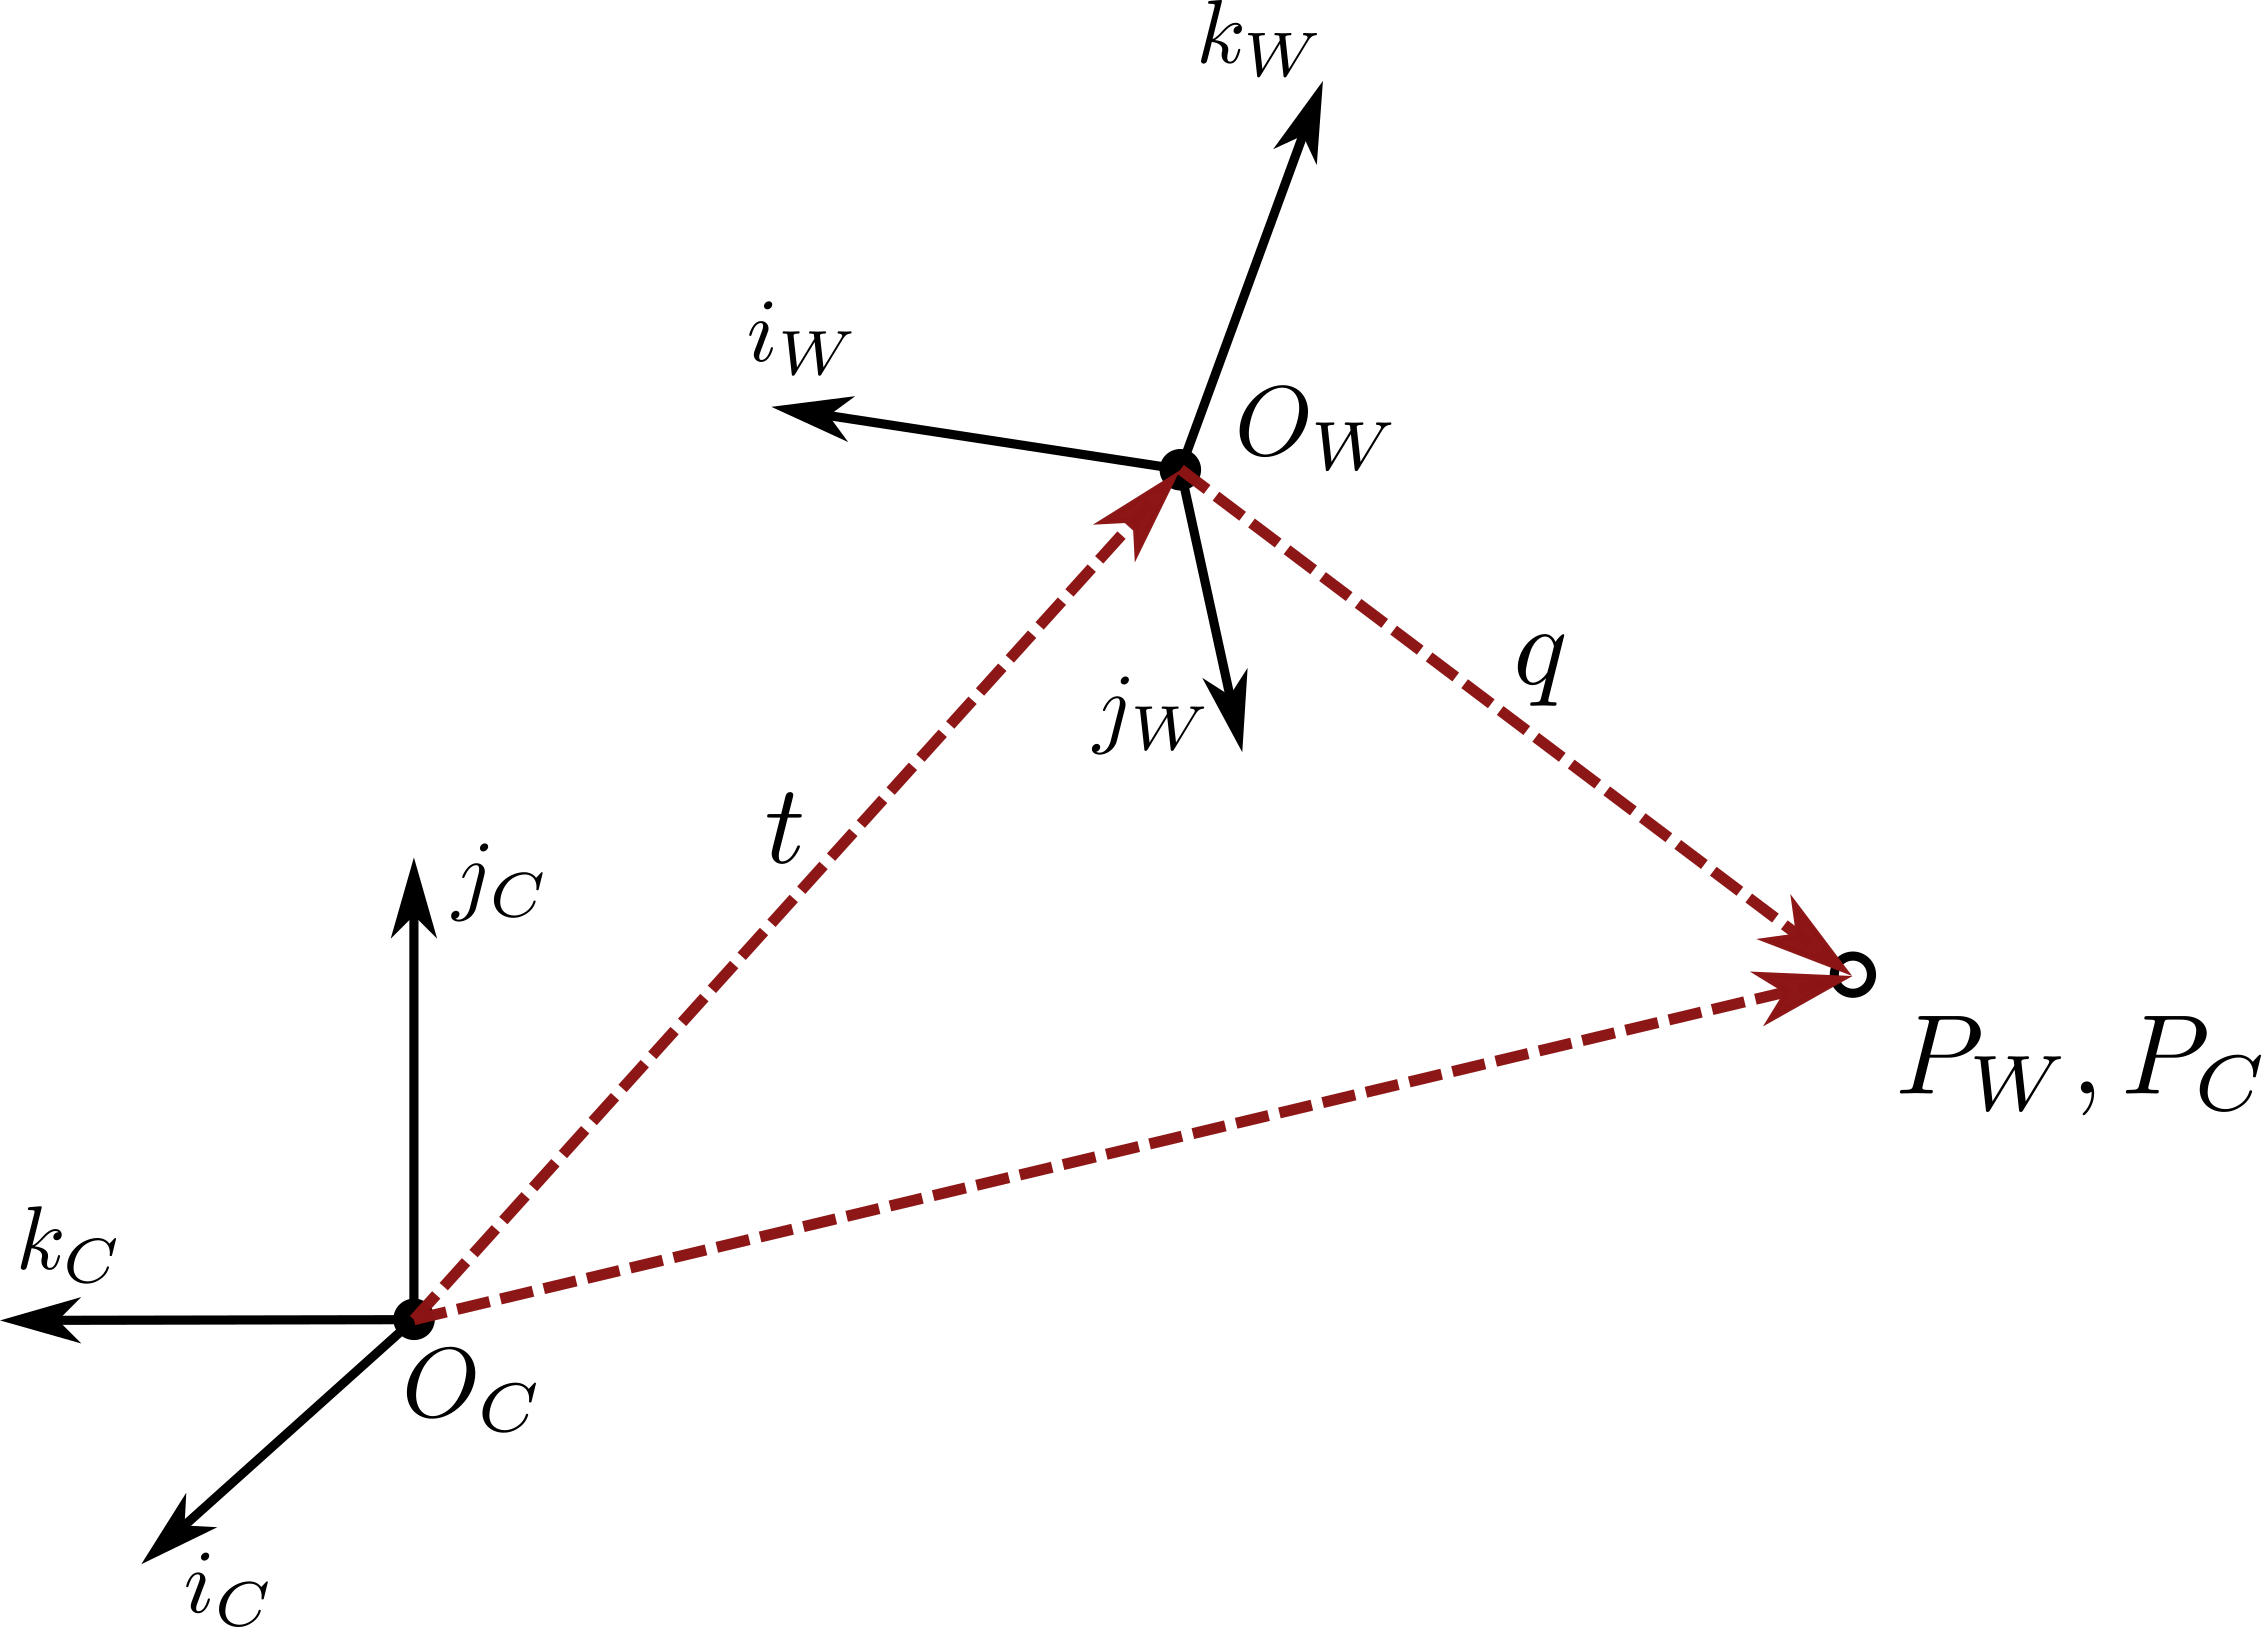
\includegraphics[width=0.65\textwidth]{tex/figs/ch09_figs/world2camera.png}
\caption{A depiction of the point $P$ expressed either in camera coordinates, $P_C$, or in world frame coordinates, $P_W$. The world frame origin is denoted by $O_W$ and the camera frame origin is denoted by $O_C$.}
\label{fig:Pc2Pw}
\end{figure}

From Figure \ref{fig:Pc2Pw} it can be seen that $P_C$ can be written as:
\begin{equation}
P_{C} = t + q,
\end{equation}
where $t$ is the vector from $O_C$ to $O_W$ expressed in camera frame coordinates and $q$ is the vector from $O_W$ to $P$ expressed in camera frame coordinates. However, the vector $q$ is in fact the same vector as $P_W$, just expressed in different coordinates (i.e. with respect to a different frame). The coordinates can be related by a rotation:
\begin{equation}
q = RP_W,
\end{equation}
where R is the rotation matrix relating the camera frame to world frame and is defined as:
\begin{equation} \label{eq:rotmatrix}
R =
\begin{bmatrix}
i_w \cdot i & j_w \cdot i & k_w \cdot i \\
i_w \cdot j & j_w \cdot j & k_w \cdot j \\
i_w \cdot k & j_w \cdot k & k_w \cdot k
\end{bmatrix},
\end{equation}
where $i$, $j$, and $k$ are the unit vectors that define the camera frame and $i_w$, $j_w$, and $k_w$ are the unit vectors that define the world frame. To summarize, the point $P_W$ can be mapped to camera frame coordinates $P_C$ as:
\begin{equation}
P_C = t + R P_W,
\end{equation}
where $t$ is the vector in camera frame coordinates from $O_C$ to $O_W$ and $R$ is the rotation matrix defined in \eqref{eq:rotmatrix}.
Similar to the previous section, these expressions can also be equivalently expressed for the case where the points $P_W$ and $P_C$ are expressed in homogeneous coordinates:
\begin{equation} \label{eq:Pw2Pchomo}
\begin{split}
\begin{pmatrix}
    P_C \\ 1
    \end{pmatrix} = \begin{bmatrix}
R & t \\
0_{1\times3} & 1
\end{bmatrix}
\begin{pmatrix}
P_W \\ 1
\end{pmatrix}.
\end{split}
\end{equation}


\subsubsection{Mapping World Frame Coordinates to Image Coordinates ($P_W \xrightarrow{} p$)}
The original objective of perspective projection was to find a way to mathematically relate the position of a point $P$ in world frame coordinates (denoted $P_W$) to the corresponding pixel coordinates $p$ on the image plane. With the relationship \eqref{eq:Pw2Pchomo} developed for mapping $P_W$ to the camera frame coordinates $P_C$, and the relationship \eqref{eq:PC2uvhomo} for mapping $P_C$ to pixel coordinates $p$, the direct mapping from $P_W$ to $p$ can now be defined. In particular, simply combining the two transformation together yields:
\begin{equation*}
p^h = \begin{bmatrix}
K \quad 0_{3\times 1}
\end{bmatrix}
\begin{bmatrix}
R && t \\
0_{1 \times 3} && 1
\end{bmatrix}
P_W^h,
\end{equation*}
which can then be simplified to:
\begin{equation} \label{eq:Pw2uvhomo}
p^h = K\begin{bmatrix}
    R & t
\end{bmatrix} P_W^h.
\end{equation}
In \eqref{eq:Pw2uvhomo}, $P_W^h$ is the homogeneous coordinate representation of $P_W$ and $p^h$ is the homogeneous coordinate representation of $p$. Additionally, recall that the matrix $K \in \mathbb{R}^{3\times3}$ is the matrix of intrinsic camera parameters, and the matrix $[R \:\:\: t] \in \mathbb{R}^{3\times 4}$ contains \textit{extrinsic} parameters (i.e. that describe the camera's position and orientation relative the points in the scene). Note that the total number of degrees of freedom is 11, where 5 are from the intrinsic parameters that define $K$, 3 are from the rotation matrix $R$, and 3 are from the position vector $t$.

\subsection{Camera Calibration: Direct Linear Method}
Before the expression \eqref{eq:Pw2uvhomo} can be used in practice, the camera's intrinsic and extrinsic parameters need to be determined (i.e. $K$, $R$, and $t$). One approach is to use the direct linear transformation method for camera calibration, which requires a set of known correspondences $p_i \xleftrightarrow[]{} P_{W,i}$ for $i = 1,\dots,n$.

\subsubsection{Direct Linear Calibration: Step 1}
First, each corresponding pair of points $p_i = (u_i,v_i)$ and $P_{W,i} = (X_{W,i}, Y_{W,i}, Z_{W,i})$ is written in homogeneous coordinates and the expression \eqref{eq:Pw2uvhomo} is used to write:
\begin{equation} \label{eq:correspondance}
    p_i^h = M P_{W,i}^h, \quad i = 1,....n
\end{equation}
where $M = K[R \:\:\: t]$ is referred to as the \textit{homography}. The first step of the camera calibration process is to use the $n$ correspondences to compute the homography $M$, and then later the intrinsic and extrinsic parameters can be extracted from $M$. To determine $M$, a useful first step is to rewrite $M$ in terms of its rows:
\begin{equation}
    M = \begin{bmatrix}
        m_1 \\ m_2 \\ m_3
    \end{bmatrix},
\end{equation}
where $m_i \in \R^{1 \times 4}$ is the $i$-th row of $M$. By considering the rows of $M$ individually, the relationship \eqref{eq:correspondance} can be written as:
\begin{equation*}
    \begin{bmatrix}
        \alpha u_i \\ \alpha v_i \\ \alpha
    \end{bmatrix} = \begin{bmatrix}
         m_1 \cdot P_{W,i}^h \\ m_2 \cdot P_{W,i}^h \\ m_3 \cdot P_{W,i}^h \\
    \end{bmatrix}, \quad i = 1,....n
\end{equation*}
which by mapping the homogeneous coordinates $p_i^h$ back to the original coordinates $p_i$ yields the $2n$ expressions:
\begin{equation*}
\begin{split}
    u_i &= \frac{m_1 \cdot P_{W,i}^h}{m_3 \cdot P_{W,i}^h}, \quad i = 1,\dots,n \\
    v_i &= \frac{m_2 \cdot P_{W,i}^h}{m_3 \cdot P_{W,i}^h}, \quad i = 1,\dots,n,
\end{split}
\end{equation*}
or equivalently (via algebraic manipulation) the expressions:
\begin{equation}
\begin{split}
    u_i(m_3 \cdot P_{W,i}^h) - (m_1 \cdot P_{W,i}^h) &= 0, \quad i = 1,\dots,n \\
    v_i(m_3 \cdot P_{W,i}^h) - (m_2 \cdot P_{W,i}^h) &= 0, \quad i = 1,\dots,n.
\end{split}
\end{equation}
Now, these $2n$ equations can be combined together in one large matrix equation:
\begin{equation}
    \tilde{P}m = 0, \quad m = \begin{bmatrix}
        m_1^T \\ m_2^T \\ m_3^T
    \end{bmatrix},
\end{equation}
where $m \in \R^{12 \times 1}$ is a vector consisting of the stacked rows of $M$ and $\tilde{P} \in \R^{2n \times 12}$ is a matrix of \textit{known} coefficients determined by the quantities $u_i$, $v_i$, and $P^h_{W,i}$. For a more concrete representation of how $\tilde{P}$ is defined, the first couple rows are given by:
\begin{equation} \label{eq:Pmeq}
\tilde{P} =
     \begin{bmatrix}
  -(P_{W,1}^h)^T & 0_{1\times 4} & u_{1} (P_{W,1}^h)^T \\
  0_{1 \times 4} & -(P_{W,1}^h)^T & v_{1} (P_{W,1}^h)^T  \\
  -(P_{W,2}^h)^T & 0_{1\times 4} & u_{2} (P_{W,2}^h)^T \\
  \vdots & \vdots & \vdots
 \end{bmatrix}.
\end{equation}
Note that $n \geq 6$ (i.e. at least 6 correspondences have been made) is a requirement to ensure that $m$ can be uniquely defined. Ideally, with this sufficient number of correspondences the equation \eqref{eq:Pmeq} could be directly solved. However, in practice a more robust procedure is to build $\tilde{P}$ with more than 6 points, which would lead to an overdetermined set of equations that may not have a solution\footnote{This is particularly true in real-world applications where noise corrupts the data.}! 
Therefore, the determination of $m$ is accomplished by formulation the optimization problem:
\begin{equation} \label{eq:mopt}
\begin{split}
\underset{m}{\text{min.}} \:\:& \lVert \tilde{P} m \rVert^2, \\
    \text{s.t.}\:\:& \lVert m \rVert^2 = 1,
\end{split}
\end{equation}
where the constraint $\lVert m \rVert^2 = 1$ is required to ensure that the optimization problem does not simply choose $m_i=0$ for each $i = 1,\dots,12$. This optimization problem is called a \textit{constrained least-squares} problem.

\begin{example}[Constrained Least-Squares] \label{ex:constlsq}
\theoremstyle{definition}
The constrained least squares problem 
\begin{equation*}
\begin{split}
\underset{x}{\text{min.}} \:\:& \lVert A x \rVert^2, \\
    \text{s.t.}\:\:& \lVert x \rVert^2 = 1,
\end{split}
\end{equation*}
with $x\in \R^n$ and $A \in \R^{m \times n}$ and $m > n$ is a finite-dimensional optimization problem. Consider the corresponding Lagrangian:
\begin{equation*}
L = x^T A^TAx + \lambda (1 - x^Tx),
\end{equation*}
and the necessary optimality conditions:
\begin{equation*}
\begin{split}
\nabla_x L &= 2(A^TA - \lambda I)x = 0, \\
\nabla_\lambda L &= 1 - x^Tx = 0. \\
\end{split}
\end{equation*}
The first NOC can be rewritten as $A^TA x = \lambda x$, and therefore any $x$ that satisfies this condition must be an eigenvector of the matrix $A^TA$. Additionally, while all the eigenvectors satisfy this condition the minimizer is the eigenvector associated with the smallest eigenvalue.
This eigenvector can efficiently be computed by a singular value decomposition of $A = U\Sigma V^T$ and then choosing $m$ to be the column of $V$ associated with the smallest singular value (since $A^TA = V\Sigma^2 V^T$).
\end{example}

\subsubsection{Direct Linear Calibration: Step 2}
Once the optimization problem \eqref{eq:mopt} has been solved for $m$ the homography $M$ is completely defined. The next step in the camera calibration process is to extract the intrinsic and extrinsic camera parameters from the matrix $M$. For this section the matrix $M$ is expressed in terms of its columns:
\begin{equation*}
M = \begin{bmatrix}
    c_1 & c_2 & c_3 & c_4
\end{bmatrix},
\end{equation*}
where $c_i$ is the $i$-th column of $M$. It is now possible to factorize $M$ as:
\begin{equation}
    M = K\begin{bmatrix}
        R & t
    \end{bmatrix},
\end{equation}
by taking the first three columns of $M$ and performing a \textit{RQ factorization}:
\begin{equation}
\begin{bmatrix}
    c_1 & c_2 & c_3
\end{bmatrix} = KR,
\end{equation}
where $R$ is an orthogonal matrix and $K$ is an upper triangular matrix. Once $K$ is known the vector $t$ can be computed by $t = K^{-1} c_4$.

\subsubsection{A Flexible Camera Calibration Method (Zhang, 2000):} \label{subsubsec:zhang}
The homography $M$ is defined for a \textit{specific} set of extrinsic parameters $R$ and $t$. In practice it might be desirable to estimate the camera's intrinsic parameters from $N$ \textit{different} images from different perspectives (and therefore with $N$ different homographies). In this case the procedure described in \cite{Zhang2000} can be used to extract the intrinsic parameters $K$. 

This approach begins by assuming that the known points $P_W$ for each individual image lie on a plane. For example the calibration ``scene'' might consist of a pattern (e.g. a checkerboard pattern) on a planar surface. In this case, it can simply be assumed that the world frame origin also lies on this plane such that $Z_W = 0$ for all points on the plane. Since $Z_W = 0$ the relationship between $p^h$ and $P^h_W$ given by \eqref{eq:Pw2uvhomo} can be simplified to:
\begin{equation}
p^h = \tilde{M} \tilde{P}_W^h,
\end{equation}
with
\begin{equation}
    \tilde{M} = K\begin{bmatrix}
    r_1 & r_2 & t
\end{bmatrix}, \quad \tilde{P}_W^h = \begin{bmatrix}
    X_W & Y_W & 1
\end{bmatrix}^T,
\end{equation}
where $\tilde{M}$ is the simplified homography matrix, $\tilde{P}_W^h$ is the simplified position of the point $P$ in world frame written in homogeneous coordinates, and $r_i$ is the $i$-th column of the rotation matrix $R$. Note that the homography matrix $\tilde{M}$ can still be estimated using the same procedure discussed before.

A set of constraints on the intrinsic parameter matrix $K$ are next identified by writing the homography $\tilde{M}$ as:
\begin{equation*}
    \begin{bmatrix}
        \tilde{c}_1 & \tilde{c}_2 & \tilde{c}_3
        \end{bmatrix} = \begin{bmatrix}
        Kr_1 & Kr_2 & Kt
    \end{bmatrix}.
\end{equation*}
This relationship, and the knowledge that $r_1$ and $r_2$ are orthonormal, leads to the following constraints:
\begin{equation} \label{eq:zhangconst}
    \tilde{c}_1^T B \tilde{c}_2 = 0, \quad \tilde{c}_1^T B \tilde{c}_1 = \tilde{c}_2^T B \tilde{c}_2,
\end{equation}
where $B = K^{-T}K^{-1} \in \R^{3 \times 3}$ is a \textit{symmetric} matrix. Solving for the intrinsic camera parameters $K$ can therefore be accomplished by using the constraints \eqref{eq:zhangconst} to solve for the symmetric matrix $B$, and then to use the definition of $B$ to back out the parameters that define $K$.

Several useful tricks can be employed to compute the matrix $B$ from the constraints \eqref{eq:zhangconst}. The main trick is to notice that even though $B$ consists of nine parameters, since it is symmetric only six parameters are required to fully specify it. Therefore $B \in \R^{3\times 3}$ is reparameterized as a vector $b \in \R^6$ as:
\begin{equation}
    b = \begin{bmatrix}
        B_{11} & B_{12} & B_{22} & B_{13} & B_{23} & B_{33}
    \end{bmatrix}^T.
\end{equation}
This reparameterization is useful because it allows us to rewrite the expression $\tilde{c}_i^TB\tilde{c}_j$ as:
\begin{equation}
    \tilde{c}_i^TB\tilde{c}_j = v_{ij}^T b,
\end{equation}
where:
\begin{equation*}
\begin{split}
   v_{ij} = \begin{bmatrix}
        \tilde{c}_{i1}\tilde{c}_{j1}, & \tilde{c}_{i1}\tilde{c}_{j2}+\tilde{c}_{i2}\tilde{c}_{j1}, & \tilde{c}_{i2}\tilde{c}_{j2}, & \tilde{c}_{i3}\tilde{c}_{j1} + \tilde{c}_{i1}\tilde{c}_{j3}, & \tilde{c}_{i3}\tilde{c}_{j2} + \tilde{c}_{i2}\tilde{c}_{j3}, & \tilde{c}_{i3}\tilde{c}_{j3}
    \end{bmatrix}^T,
\end{split}
\end{equation*}
where $\tilde{c}_{ik}$ is the $k$-th element of the column vector $\tilde{c}_i$ and $\tilde{c}_{jk}$ is the $k$-th element of the column vector $\tilde{c}_j$. With this reparameterization, the constraints \eqref{eq:zhangconst} can be rewritten as:
\begin{equation*}
\begin{split}
\tilde{c}_1^T B \tilde{c}_2 = 0 &\implies v_{12}^Tb = 0 \\
\tilde{c}_1^T B \tilde{c}_1 = \tilde{c}_2^T B \tilde{c}_2 &\implies (v_{11} - v_{22})^T b = 0,
\end{split}
\end{equation*}
or by combining them:
\begin{equation} \label{eq:bconst}
    \begin{bmatrix}
        v_{12}^T \\ (v_{11} - v_{22})^T
    \end{bmatrix}b = 0,
\end{equation}
which is linear in the unknowns $b$. Importantly, while the homographies $M$ are different for each image, the intrinsic camera parameters (i.e. the vector $b$) are the same! Therefore for $N$ images from the same camera (but with potentially different perspectives) these constraints \eqref{eq:bconst} can be stacked to give:
\begin{equation} \label{eq:allbconst}
    Vb = 0,
\end{equation}
where $V \in \R^{2N \times 6}$. In the case where the skewness parameter $\gamma$ is included in $K$ there must be $N \geq 3$ images in order to specify $B$ uniquely. Similar to how the homography for an image $M$ was computed in the previous section, the vector $b$ will be specified by the solution to the constrained least squares problem:
\begin{equation} \label{eq:bopt}
\begin{split}
\underset{b}{\text{min.}} \:\:& \lVert Vb \rVert^2, \\
    \text{s.t.}\:\:& \lVert b \rVert^2 = 1.
\end{split}
\end{equation}
Once $b$ has been determined, the intrinsic camera parameters $K$ can be solved for recalling the definition of $B = K^{-T}K^{-1}$. In particular, the intrinsic parameters are given by:
\begin{equation} \label{eq:B2K}
\begin{split}
    v_0 &= \frac{B_{12}B_{13} - B_{11}B_{23}}{B_{11}B_{22} - B_{12}^2}, \\
    \lambda &= B_{33} - \frac{B_{13}^2 + v_0(B_{12}B_{13} - B_{11}B_{23})}{B_{11}}, \\
    \alpha &= \sqrt{\frac{\lambda}{B_{11}}}, \\
    \beta &= \sqrt{\frac{\lambda B_{11}}{B_{11}B_{22} - B_{12}^2}}, \\
    \gamma &= \frac{-B_{12}\alpha^2\beta}{\lambda}, \\
    u_0 &= \frac{\gamma v_0}{\beta} - \frac{B_{13}\alpha^2}{\lambda},
\end{split}
\end{equation}
where $\lambda$ can be though of as a scaling parameter that accounts for the fact that there are five unknown camera intrinsic parameters but six degrees of freedom in $B$.

Once the camera intrinsic parameters $K$ have been extracted from this procedure, given any new homography $\tilde{M}$ the extrinsic parameters can be computed by:
\begin{equation}
\begin{split}
    r_1 &= \frac{K^{-1}\tilde{c}_1}{\lVert K^{-1}\tilde{c}_1 \rVert}, \\
    r_2 &= \frac{K^{-1}\tilde{c}_2}{\lVert K^{-1}\tilde{c}_2 \rVert}, \\
    r_3 &= r_1 \times r_2, \\
    t &= \frac{K^{-1}\tilde{c}_3}{\lVert K^{-1}\tilde{c}_1 \rVert}.
\end{split}
\end{equation}
As one final step, it is noted that the matrix $R$ defined with columns $r_1$, $r_2$, and $r_3$ will not in generally satisfy the properties of a rotation matrix (i.e. orthonormality). One final step to this overall procedure is to correct this issue by finding the rotation matrix that best corresponds to these column vectors. This is accomplished again by optimization, and in particular by formulating the problem:
\begin{equation} \label{eq:Ropt}
\begin{split}
\underset{R}{\text{min.}} \:\:& \lVert R - Q \rVert^2, \\
    \text{s.t.}\:\:& R^TR = I,
\end{split}
\end{equation}
where
\begin{equation*}
    Q = \begin{bmatrix}
        r_1 & r_2 & r_3
    \end{bmatrix}.
\end{equation*}
This problem is solved by choosing $R = UV^T$ where $U$ and $V$ are defined by the singular value decomposition of $Q = U\Sigma V^T$.

\subsection{Limitations}

\subsubsection{Radial Distortion}
The pinhole camera model provides a nominal camera model for which it is relatively straightforward to develop a mathematical model of the perspective projection. However, in practice this model is not a perfect representation of the imaging process. One such effect that is not captured by the pinhole model is \textit{radial distortion}, which is an effect seen in real lenses where either barrel distortion or pincushion distortion will affect the real pixel coordinates. Images showing both barrel and pincushion distortion are provided in Figure \ref{fig:distortion}.

\begin{figure}[ht]

\includegraphics[width=0.75\textwidth]{tex/figs/ch09_figs/lensdistortion.png}
\centering
\caption{Different kinds of radial distortions that are seen in real lenses, which may affect the accuracy of the pinhole camera model.}
\label{fig:distortion}
\end{figure}

There are methods that can be used to correct for image distortion. A simple and efficient way is to model the relationship between the ideal pixel coordinates $(u,v)$ and the distorted pixel coordinates $(u_d,v_d)$ as:
\begin{equation}
\begin{bmatrix}
    u_d \\
    v_d
\end{bmatrix}
=
\begin{bmatrix}
    u_d \\
    v_d
\end{bmatrix}
(1+kr^2)
\begin{bmatrix}
    u-u_{cd} \\
    v-v_{cd}
\end{bmatrix}
+
\begin{bmatrix}
    u_{cd} \\
    v_{cd}
\end{bmatrix}
\end{equation}
where $k \in \mathbb{R}$ is the radial distortion factor, $(u_{cd}, v_{cd})$ are the pixel coordinates of the image center, and $r^2=(u-u_{cd})^2+(v-v_{cd})^2$ is the square of the distance between the ideal pixel location and the center of distortion.. Note that $k$ differs in different cameras and needs to be pre-determined.

\subsubsection{Measuring Depth}
Once the camera intrinsic and extrinsic parameters $K$, $R$, and $t$ are known it is still not possible to map pixel coordinates to the corresponding point in space. Mathematically this is a result of the matrix $M$ in \eqref{eq:correspondance} not being invertible, but intuitively this is because the distance along the line of sight from $p$ to $P$ in Figure \ref{fig:pinhole_cam} can not be determined!

However, there are some techniques that can enable depth estimates to be made with a single camera. One approach is known as \textit{depth from focus}, where several images are taken until the projection of point $P$ is in focus. Based on the thin lens model, when this occurs:
\begin{equation*}
    \frac{1}{z} + \frac{1}{Z} = \frac{1}{f},
\end{equation*}
where $f$ is the focal length, $Z$ is the depth of the point $P$ in camera frame, and $z$ is the depth of the image plane in the camera frame when the projection of point $P$ is in focus. Since $f$ and $z$ are known, the depth $Z$ can therefore be computed.
If two cameras are used, depth estimation is possible via \textit{binocular reconstruction} or \textit{stereo vision}. This approach requires known corresponding pixel coordinates $p$ and $p'$ of each camera, and then uses \textit{triangulation} to determine the 3D position of the source point $P$ in the scene.

\subsection{Exercises}
\subsubsection{Camera Calibration}
Complete \textit{Problem 1: Camera Calibration} located in the online repository:

\vspace{\baselineskip}

\url{https://github.com/PrinciplesofRobotAutonomy/AA274A_HW3},

\vspace{\baselineskip}

where you will estimate the intrinsic parameters of a camera using the method described in Section \ref{subsubsec:zhang}.
